\subsection{Architettura del Ranking Service}
\subsubsection{Descrizione}
Il microservizio denominato \textit{Ranking Service} svolge le seguenti funzionalità:
\begin{itemize}
	\item Gestione della classifica: ogni volta che un nuovo messaggio () viene aggiunto alla coda SQS, viene chiamati il metodo \texttt{refresh\_ranking} che si occupa di recuperare e fare la parsificazione e deserializzazione dei messaggi nella coda (lavorando a batch di massimo 10 messaggi). Dopo di che i messaggi vengono analizzati tramite i servizi Comprehend\glo e Rekognition\glo di AWS e vengono generati i punteggi per le foto, per il testo e per le emoji. Viene quindi aggiornato il database, aggiungendo il ristorante e il media (se non presenti) e aggiornati i punteggi.
	Vengono inoltre esposti due API endpoint:
		\begin{itemize}
			\item \texttt{getRanking}: restituisce una parte della classifica generale;
			\item \texttt{getLabelAndPost}: restituisce i media (e le relative label\glo) di un particolare ristorante.
		\end{itemize}
	\item Funzionalità di ricerca: viene esposto un API endpoint \texttt{searchByName} che restituisce tutte le informazioni presenti nel database relative ad un ristorante con un nome specifico (media compresi); 
	\item Gestione dei preferiti: viene esposto un API endpoint \texttt{favorites} che abilità alla gestione della lista di ristoranti preferiti per ogni utente, fornendo le funzionalità di aggiunta, rimozione e visualizzazione per la lista dei preferiti.
\end{itemize}

\subsubsection{Diagrammi delle classi}
\begin{figure}[H]
    \centerfloat
    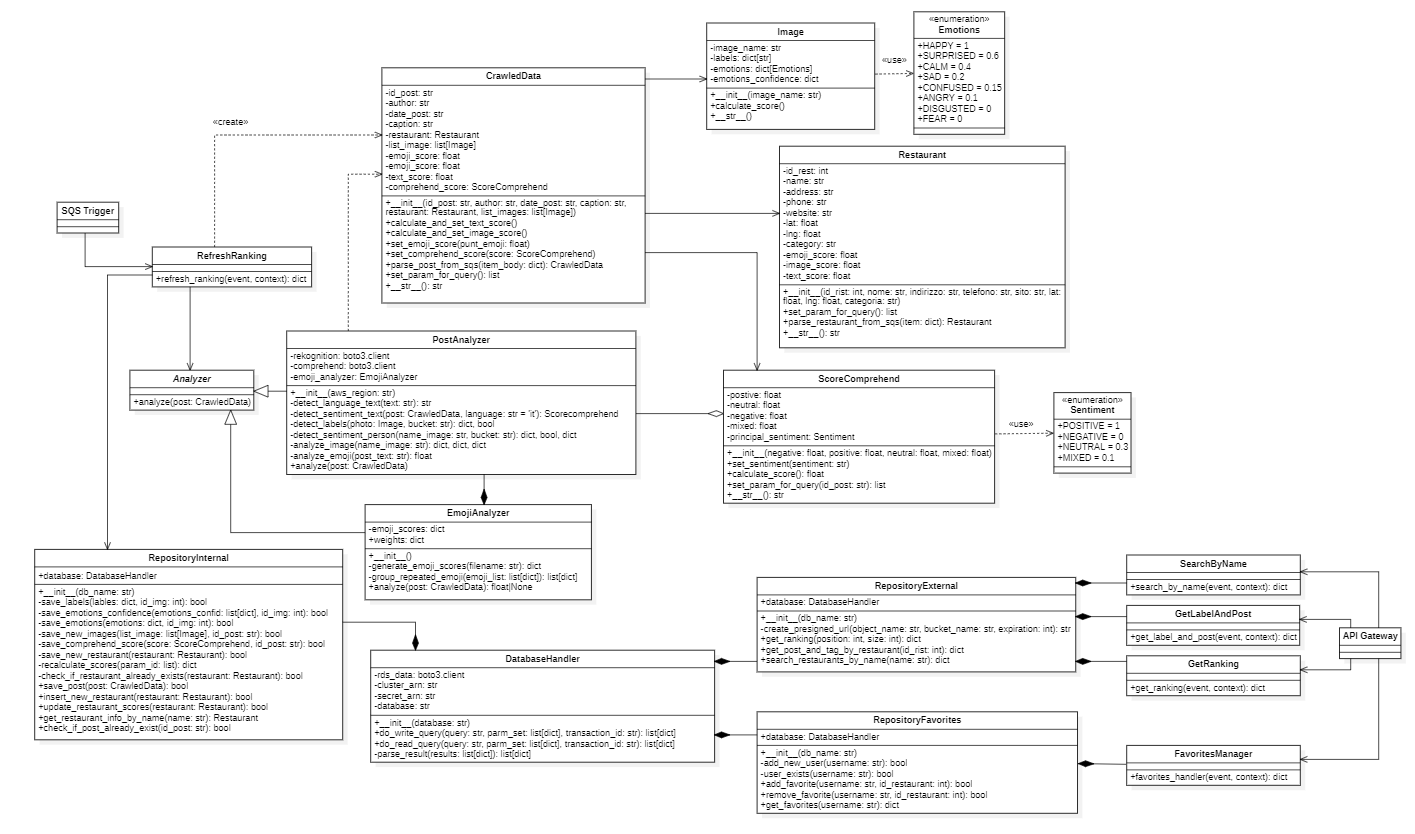
\includegraphics[scale=0.35]{Contenuto/Immagini/classi-RS.png}
    \caption{Ranking Service - Diagramma delle classi}
\end{figure}

\subsubsection{Diagrammi di sequenza}
In questa sezione vengono presentati i diagrammi di sequenza che modellano le operazioni principali del Ranking Service:
\begin{itemize}
	\item Il processo di analisi di un media, assumendo che il media e il ristorante non siano già presenti nel database e che siano presenti persone delle immagini;
	\item Il processo di salvataggio del media analizzato e del ristorante, sempre assumendo che il media e il ristorante non siano già presenti nel database, e l'aggiornamento dei punteggi.
\end{itemize}
\begin{figure}[H]
    \centerfloat
    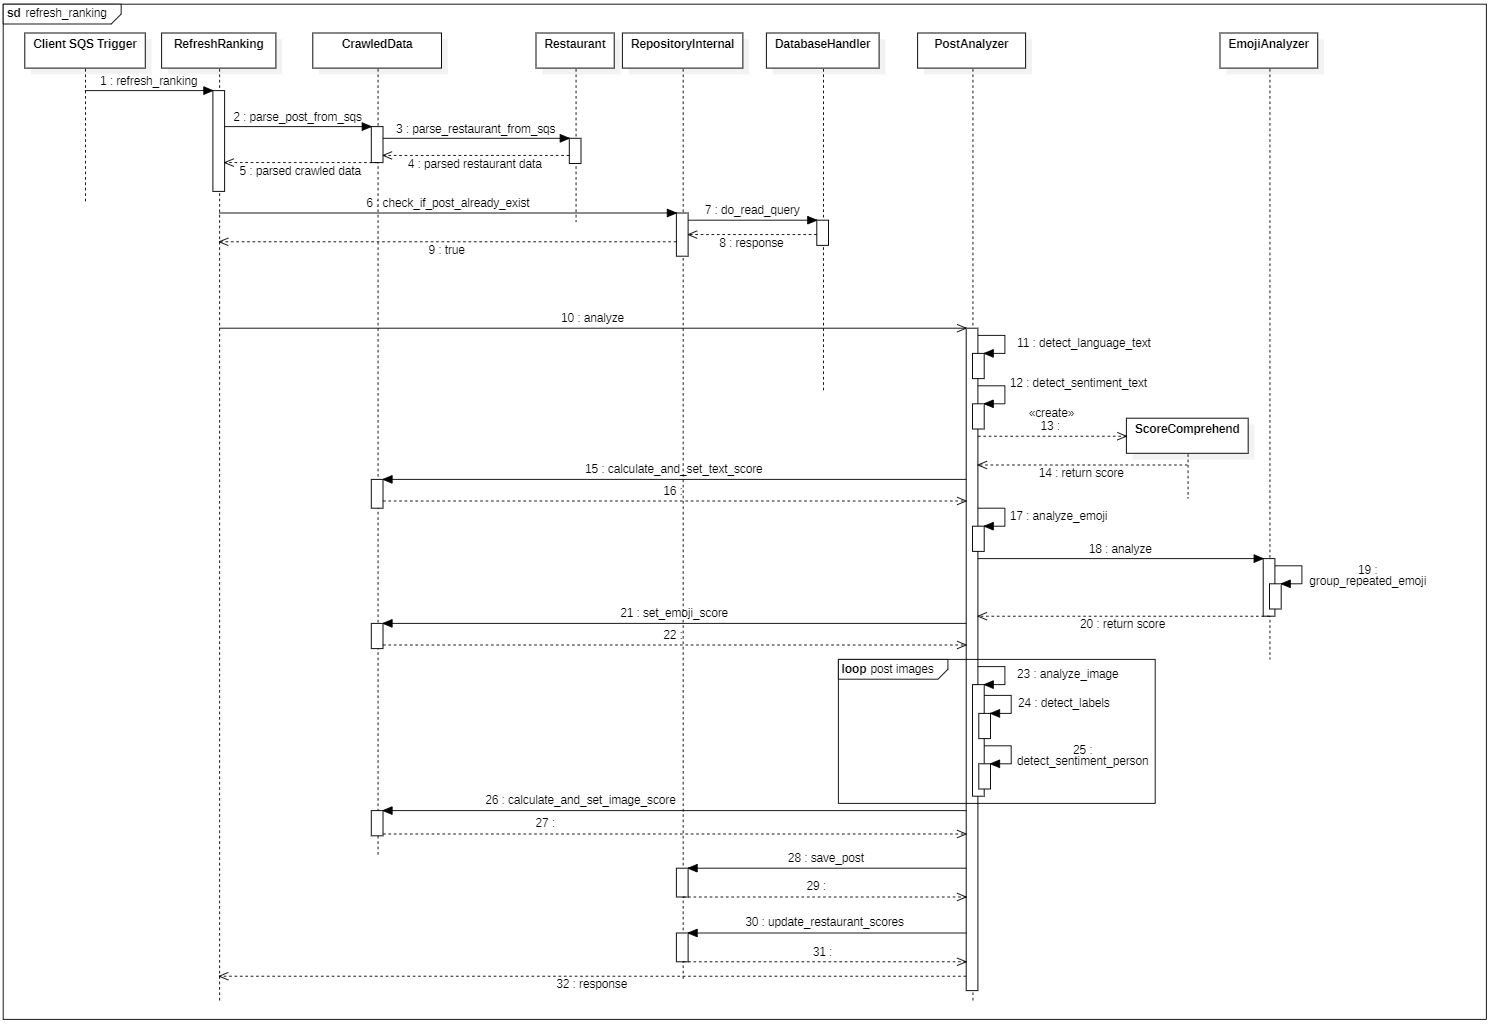
\includegraphics[scale=0.45]{Contenuto/Immagini/seq1-RS.JPG}
    \caption{Ranking Service - Diagramma di sequenza - 1}
\end{figure}
\begin{figure}[H]
    \centering
    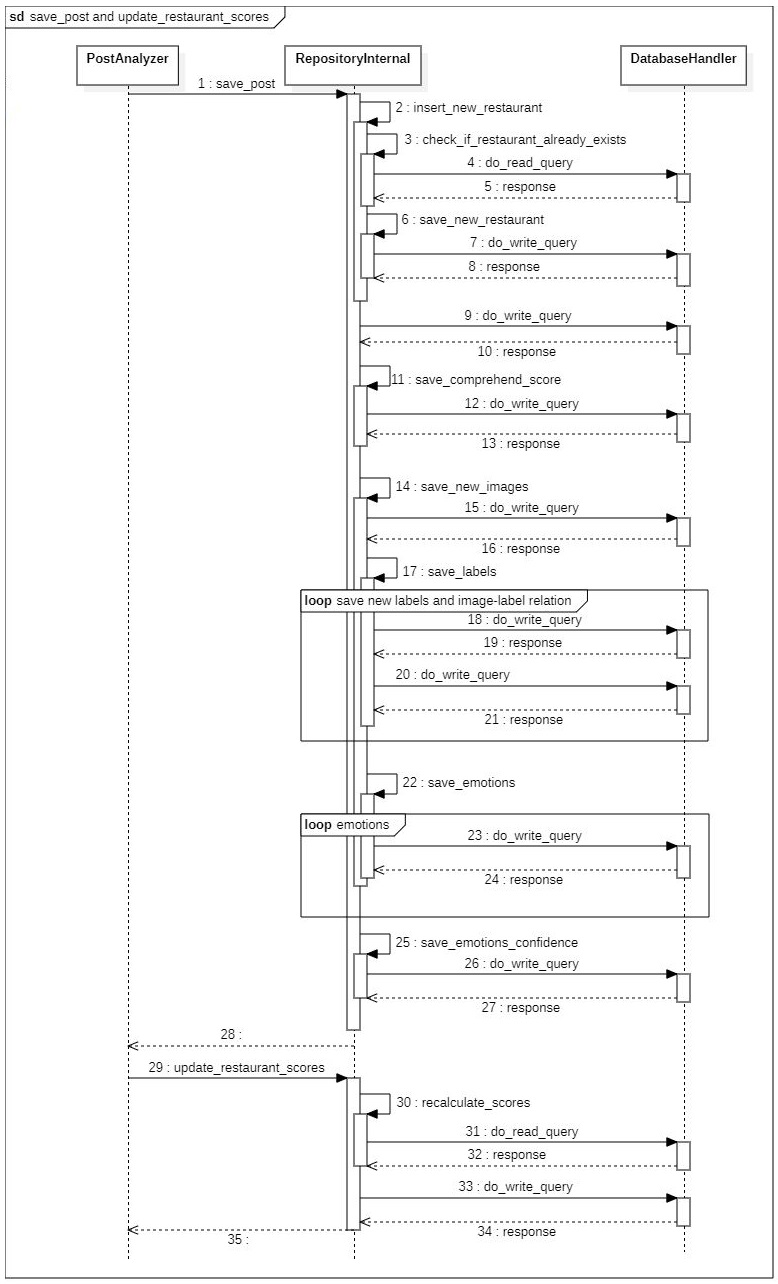
\includegraphics[scale=0.55]{Contenuto/Immagini/seq2-RS.JPG}
    \caption{Ranking Service - Diagramma di sequenza - 2}
\end{figure}

\subsubsection{Note sul processo di analisi}
Dopo alcune prove ed osservazioni sono state fatte alcune decisioni relative al processo di analisi:
\begin{itemize}
	\item Dopo l'analisi della immagini, verranno salvate nel database solo le label relative al cibo (quindi con padre "Food") e con confidenza di almeno il 90\%;
	\item Solo se nelle immagini viene trovata la label "Person" verrà effettuata l'analisi dei sentimenti nell'immagine tramite Rekognition, anche in questo caso verranno salvati solo i sentimenti predominanti con una confidenza di almeno il 90\%.
\end{itemize}

\subsubsection{Design pattern notevoli utilizzati}
Per La realizzazione del Ranking Service sono stati utilizzati i seguenti design pattern:
\begin{itemize}
    \item \textbf{Strategy:} Utlizzato per la realizzazione di PostAnalyzer ed EmojiAnalyzer, è stato scelto principalmente per la sua versatilità.\\
    Questo pattern infatti ci permette, nel caso in cui in futuro ci sia bisogno di un algoritmo più avanzato per l'analisi dei post, con il minimo sforzo e modifica del codice, di implementare la nuova classe che erediterà anch'essa dalla classe base Analyzer.
    \item \textbf{Static Factory:} Utilizzato per la creazione di oggetti dalle varie fonti accessibili dal microservizio, come la coda SQS, e la creazione di liste contenti dati pronti per l'utilizzo nei metodi riguardanti il database.
\end{itemize}

\subsubsection{Schema del database}
\begin{figure}[h]
    \centering
    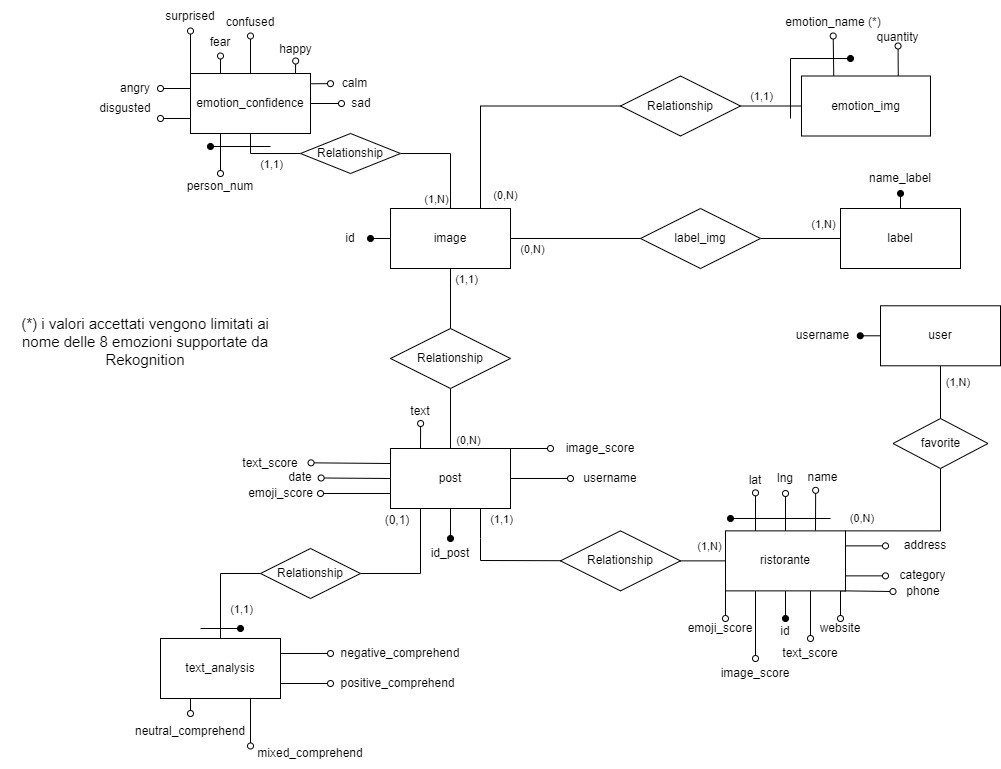
\includegraphics[scale=0.35]{Contenuto/Immagini/ER-RS.jpg}
    \caption{Ranking Service - Schema ER del database}
\end{figure}